\input{chapter-header.tex}

% ===========================================================================
\chapter{\VTT: Virtualized Application Runtimes}
\chaplabel{vtt}
\minitoc
% ===========================================================================
\introduction
% ===========================================================================

This chapter presents our Virtualization Application Runtime infrastructure, namely \VTT. It focuses on the model of our solution and presents its core ideas. \VTT supports application runtime virtualization through two key ideas:

\begin{description}
\item[Application co-location.] The ability to have co-existing applications on top of the same virtual machine. 
\item[Object spaces.] An object space is a first-class application runtime. It encapsulates the access to an application runtime and provides a high-level API to easily query and manipulate it.
\end{description}

In \Vtt two co-existing application runtimes have two well-defined roles. The \emph{virtualized} runtime is the application runtime under manipulation. The \emph{hypervisor} controls and manipulates the virtualized runtime~(cf. Section \ref{sec:virtualization_overview}) through the object space.
Figure \ref{fig:virtualization_introduction} shows a simplified schema of the solution.

\begin{figure}[htb]
\begin{center}
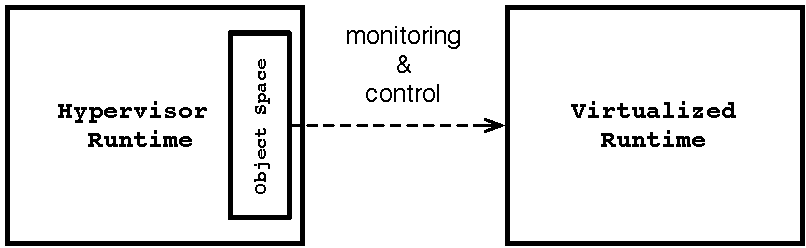
\includegraphics[width=.8\linewidth]{virtualization_introduction}
\caption{\textbf{Virtualization concepts in \Vtt.} Two co-existing application runtimes with two well-defined roles.\label{fig:virtualization_introduction}}
\end{center}
\end{figure}

A hypervisor can perform four basic kind of manipulations on the virtualized runtime, each with its own tradeoffs. First, it can directly manipulate its state through the object space interface~(cf. Section \ref{sec:object_space}). The other three manipulation mechanisms are based on this direct manipulation. Second, it can hook into the execution of the virtualized runtime to execute its own code~(cf. Section\ref{sec:hypervisor}). Third, we can execute arbitrary expressions inside a virtualized runtime through process injection and virtual interpretation~(Section \ref{sec:isolation}). % can execute isolated and their result can be cleanly retrieved by the hypervisor~(Section \ref{sec:isolation}). Finally, it can execute code inside an object space through a virtual code interpreter, providing full intercession power over the execution of the virtualized application for usages such as tracing or debugging~(Section \ref{sec:interpretation}).


%Although being isolated, \Vtt presents a richer message-based communication channel. The hypervisor can perform cross-runtime message-sends by injecting processes. Injected processes can execute isolated and their result can be cleanly retrieved by the hypervisor~(Section \ref{sec:isolation}).
%Additionally, a more granular control can be made through virtual execution. A specialized code interpreter provides full intercession power over the execution of the virtualized application for usages such as tracing or debugging~(Section \ref{sec:interpretation}).

%On one side, this means that the hypervisor can freely manipulate the virtualized language runtime without affecting itself. On the other side, this no-sharing strategy poses an extra effort in communication~(cf. Section \emph{sec:isolation}) mainly in object marshaling.

%A language hypervisor is a first-class object in \VTT, meaning that we can easily modify it and replace it by another object. Additionally, a simulation mode allows a fully-managed execution mode.

%We do not require any changes in existing applications to import them inside an object space. We introduce minimal modifications at the \VM level to ensure their control and manipulation is transparent. Regarding execution, an object space provides with different means for controlling the execution of the language runtime it owns~(cf. Section \ref{sec:execution}). It can safely start, pause and resume its execution, create new threads or finalize existing ones.  


\section{Controlling Virtualized Runtimes in \Vtt} \label{sec:virtualization_overview}

\Vtt presents an architecture where multiple application runtimes co-exist independently from each other. An application runtime fulfills a role inside the virtualization infrastructure. An \emph{hypervisor} monitors and controls \emph{virtualized} application runtimes. Both the virtualized runtime and the hypervisor are full-fledged high-level application runtimes. On one hand, the virtualized application runtime is written in a high-level language as the focus of this thesis is the virtualization of such runtime. Although, we would like to emphasize that the hypervisor is as well written in a high-level language~(in contrast with \eg JVMTI\cite{JVMPI}), bringing three main benefits to our solution:

\begin{description}
\item[Expressiveness and abstraction.] We can use the expressiveness and abstraction power supported by a high-level language to describe a hypervisor. For example, an hypervisor written in the Pharo language can benefit from the usage of inheritance, polymorphism and traits amongst others.
\item[Infrastructure.] The hypervisor can use all the infrastructure already available to our high-level language. It can access existing libraries such as collections, sockets and files. It also benefits from the infrastructure provided by the \VM such as automatic memory management.
\item[Tools.] We can use the same tools that we use to describe our high-level language to manipulate our hypervisor. This means that we can benefit from code browsers, refactorings, unit tests and other existing tools.
\end{description}


A first-class object space resides inside the hypervisor and represents the virtualized runtime. A hypervisor object uses the object space and implements a particular manipulation on it \eg runtime update, failure detection, browsing or debugging. Figure \ref{fig:objectSpaceOverview_architecture} provides an overview of the \Vtt's architecture.

\begin{figure}[ht]
\begin{center}
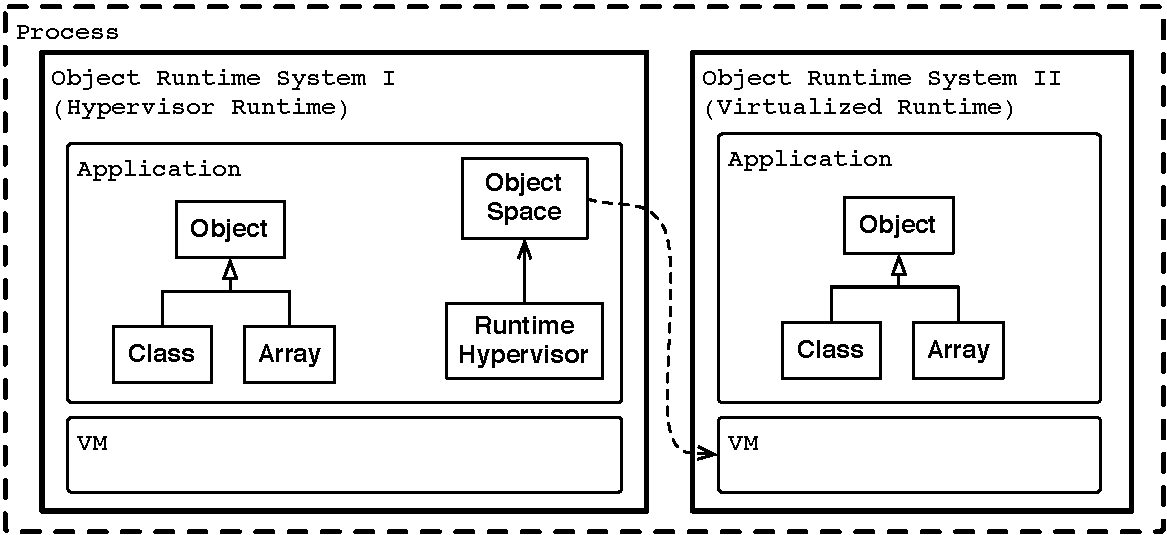
\includegraphics[width=.9\linewidth]{object_space_overview3}
\caption{\textbf{\VTT Coexistence.} The hypervisor controls the virtualized runtime through an object space.\label{fig:objectSpaceOverview_architecture}}
\end{center}
\end{figure}


Notice that the hypervisor and the virtualized runtime do not share any \VM or language state \ie each one has its own interpreter, stack, classes and objects. Their object graphs are isolated from each other \eg each one has its own \ct{Object} and \ct{String} class and their own set of unique interned strings~(the symbols). This isolation strategy allows the hypervisor to change any part of the virtualized runtime without affecting itself, as it happens in reflective architectures. From the virtualized runtime point of view, all modifications come and are applied from the outside~(the hypervisor), in contrast with reflective architectures where such changes are applied from within the application runtime under modification. This separation provides \Vtt with the following properties:

\begin{description}
\item[Transparency.] Our solution does not require any changes to the applications residing inside the virtualized runtime. Thus, we can virtualize existing application runtimes without modifying them \ie \Vtt does not require virtualized applications to include particular libraries, use particular interfaces nor change their execution model.

\item[Application independence.] Our solution does not depend on the particular application inside the virtualized runtime. Different runtime hypervisors can be written for different use cases, including application specific and general ones. The limitation of this approach is, however, its dependance on the execution model imposed by the \VM. We do not change the \VM execution semantics such as the code interpreter or the method lookup.
\end{description}

\section{Object Spaces: First-class Application Runtimes} \label{sec:object_space}

An object space is a first-class representation of an object oriented application runtime, meant for its manipulation and control. An object space encapsulates an application runtime and provides a clear and explicit interface to manipulate it. This interface is split in two different kind of objects: an \ct{objectSpace} object provides general operations on the virtualized runtime; mirror objects~\cite{Brac04b} provide operations to manipulate individual objects that reside inside the virtualized runtime~(Figure \ref{fig:objectSpaceMirrors}). Specific mirrors manipulate elements with a different object-format or runtime representation to enforce their internal representation, such as the \ct{ClassMirror}.

\begin{figure}[ht]
\begin{center}
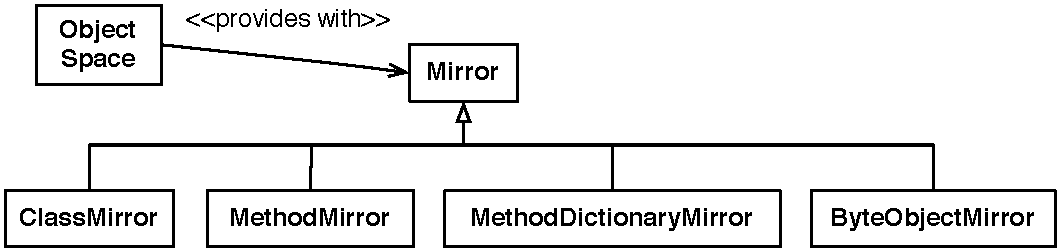
\includegraphics[width=.9\linewidth]{object_space_mirrors}
\caption{\textbf{Mirrors in Object Spaces.} An object space is the main entry point for runtime manipulation. An object space provides mirrors to modify particular objects. \label{fig:objectSpaceMirrors}}
\end{center}
\end{figure}

These objects make explicit through the operations they expose two important parts of a \VM-language interface, explained in detail in the following subsections. First, The \VM setup interface exposes the elements of the language that should be initialized so it can run a program. Second, the runtime manipulation interface exposes operations that manipulate elements/structures that live during an application's execution, such as objects, classes, threads and the execution stack.

\subsection{\VM-Setup Interface}

The \VM-setup interface is the set of bindings between the \VM and the language that the \VM needs to run a program.
For example, a \VM may need the boolean objects \ct{true} and \ct{false} to push them as the result of a boolean operation at runtime.
This configuration is usually done only during the language runtime initialization and before the execution of a program, as the \VM cannot execute it before such elements exist.
The \VM setup interface allows us to configure the following kind of elements:

\begin{description}
\item[Well-known objects of the language.] Objects such as \ct{nil}, \ct{true} or \ct{false} are needed at runtime for different purposes. For example, the garbage collection needs \ct{nil} at runtime to update weak references. Other particular objects may be held by the \VM as prototypes to speed-up instantiation time of commonly used objects.


\begin{code}
ObjectSpace {
    getNil -> Mirror
    getTrue -> Mirror
    getFalse -> Mirror

    setNil: Mirror -> Void
    setTrue: Mirror -> Void
    setFalse: Mirror -> Void
}
\end{code}

\item[Special classes.] Special classes are those needed by the \VM at runtime. They are needed to perform safety checks, create instances or handle special cases such as immediate objects. For example, when mutating a \ct{String} object the Pharo \VM checks that the introduced object is a \ct{Character} object, to avoid putting the \ct{String} into an invalid state. Also, the \VM requires references to those classes that it instantiates directly~(instead of being created through the \ct{new} message in program). For example, the Pharo \VM instantiates a \ct{BlockClosure} object when it founds the bytecodes that correspond a block expression at runtime. Finally, immediate objects are objects that are encoded inside an object reference instead of occupying extra memory inside the heap. Immediate objects include a tag in the reference that the \VM knows how to map to its corresponding class to perform the method-lookup. 

\begin{code}
ObjectSpace {
    setArrayClass: ClassMirror -> Void
    setBlockClass: ClassMirror -> Void
}
\end{code}

\item[Special messages.] Special messages are callbacks that the \VM will invoke in the application to notify particular events. The probably most known of such messages is Smalltalk's \ct{doesNotUnderstand}~(and its equivalent Ruby's \ct{methodMissing}). When the \VM does not find a method matching a message-send, it will send a \ct{doesNotUnderstand} message to the receiver object and let the user program decide what to do in such a case.

\begin{code}
ObjectSpace {
    setDoesNotUnderstandSelector: Mirror -> Void
}
\end{code}

\end{description}

This \VM setup interface avoids to hardcode particular knowledge of a language inside the \VM. This gives us the possibility to easily change particular language internals such as renaming special messages or changing the class hierarchy of special classes without leaving the virtualized runtime in an inconsistent state. Being radical, we could think about porting another language to this VM, as long as they share similar execution semantics \ie the \VM execution model is compatible with the given language and we configure this interface accordingly.


%In our particular implementation the list of classes exposed through this interface are those of literal objects and those related with the internal \VM execution model. For the sake of completeness the list of classes is the following: \ct{Array}, \ct{Association}, \ct{BlockClosure}, \ct{ByteArray}, \ct{ByteString}, \ct{ByteSymbol}, \ct{Character}, \ct{Context}, \ct{Float}, \ct{SmallInteger}, \ct{LargePositiveInteger}, \ct{LargeNegativeInteger}, \ct{Message}, \ct{CompiledMethod}, \ct{MethodDictionary}, \ct{Semaphore}, \ct{WeakFinalizationList}.

\subsection{Runtime Manipulation Interface} 
The runtime manipulation interface includes operations to monitor and modify the virtualized runtime during execution. This interface provides access to the virtualized runtime's internal elements and encapsulates implementation details behind them~(\ie the object-format imposed by the \VM). This interface provides the following kind of operations:

\begin{description}
\item[Global Access.] An object space offers operations to query and modify the global state of the virtualized runtime. For example, it provides access to the loaded classes or the running threads/processes. It exposes as well operations to install new and remove existing ones.

\begin{code}
ObjectSpace {
    "Classes"
    createClassNamed: String withFormat: Integer -> ClassMirror
    getClasses -> List<Mirror>
    getClassNamed: String -> Mirror
    removeClassNamed: String -> Void
    ...

    "Threads"
    getThreads -> List<Mirror>
    installThread: ThreadMirror -> Void
    ...
}
\end{code}

\item[Runtime Object Access.] Mirrors~\cite{Brac04b} expose operations to query or alter a particular object or element in the virtualized runtime. Different kinds of mirrors enforce the object-format of the different types of objects we can manipulate. For example, we expose specific mirrors for normal objects, classes, methods, activation records or processes. Notice that these mirrors are low-level mirrors as they expose operations to mutate and access objects in their \VM representation. Additionally, through mirrors we can execute \VM primitives on objects, providing the correct primitive ID~(an integer or native function pointer, depending on the implementation) and the corresponding arguments. These primitives are operations that the \VM exposes normally to the language.

\begin{code}
Mirror {
    "Class access"
    getClass -> ClassMirror
    setClass: ClassMirror -> Void

    "Field Access"
    getInstanceVariableNamed: String -> Mirror
    setInstanceVariableNamed: String varName withValue: Mirror -> Void
    ...
    
    "Primitive execution"
    executePrimitive: PrimitiveID withArguments: Array -> Mirror
}
\end{code}

\begin{code}
ClassMirror {
    "Instantiation"
    instantiate -> Mirror
    instantiateWithSize: Integer -> Mirror
    ...

    "Method manipulation"    
    compileMethod: String -> Void
    removeMethodNamed: String -> Void
    ...
}
\end{code}

\end{description}

% ===========================================================================

\section{First-Class Hypervisors}\label{sec:hypervisor}

The client of an object space is a \emph{hypervisor}. A hypervisor is first-class object that implements a particular monitoring/modification strategy for a virtualized runtime. For this we split a virtualized application's execution in cycles. A cycle is an execution that lasts at least a time window and finishes when it finds the next safe suspension point~(Figure \ref{fig:execution_cycle}). A safe suspension point is a point during execution where suspending a thread will not leave it in an inconsistent state. To illustrate with a concrete example, in our \Vtt prototype written for the Pharo language described in \chapref{prototype} safe suspension points are the activation of message sends and bytecode backjumps. During each execution cycle, the virtualized runtime runs unmanaged using the full \VM's capacity. When the cycle finishes because the execution completed a time window and found a suspension point, the control is given to the hypervisor. The hypervisor can monitor and modify the virtualized application at this point and then resume the execution of the virtualized runtime from the last suspension point.

\begin{figure}[ht]
\center
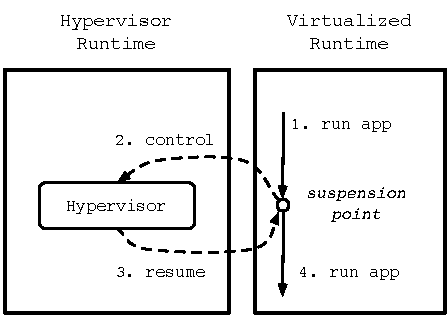
\includegraphics[width=.6\linewidth]{execution_cycle}
\caption{\textbf{Execution Cycle.} \label{fig:execution_cycle}}
\end{figure}

To enable cycle execution, the \ct{objectSpace} interface allows us to execute an application runtime during a cycle of time. An \Vtt implementation should additionally include support for suspension points. This operation will wake up the virtualized runtime processes and execute them for at least a given time. Once the cycle is finished, it will be suspended in the next suspension point it finds and the control will return to the hypervisor.

\begin{code}
ObjectSpace {
    runCycle -> Void
}
\end{code}

%Our implementation presents an execution cycle of 200ms that allows us to have fine grained control while the virtualized application has still place to run. We use as suspension points backjumps found in the executed bytecode and message sends. In such a way, we ensure that the execution stack is in a consistent state after it is interrupted.

Then, our hypervisor class hierarchy presents four basic methods. First, the \ct{run} template method implements the basics of the hypervision cycle: it resumes the execution of the virtualized runtime inside a loop. Two methods~(\ct{before} and \ct{after}) provide hooks for the specific hypervisor implementations. Figure \ref{fig:hypervisors} shows a class hierarchy example and code with two sketched hypervisors. A \ct{NullHypervisor} allows the virtualized runtime to run without any intervention. The \ct{UpdateHypervisor} instead checks the existence of a file with updates on every cycle.

\begin{code}
Hypervisor >> run
    [ true ] whileTrue: [
        self before.
        self basicRun.
        self after.
    ]

Hypervisor >> basicRun
    objectSpace runCycle.

NullHypervisor >> before
    "Nothing"

NullHypervisor >> after
    "Nothing"

UpdateHypervisor >> before
    self checkForUpdate.

UpdateHypervisor >> checkForUpdate
    "We check if a given file exists"
    'update.txt' asFile exists ifTrue: [ ...
    ...
\end{code}

\begin{figure}[ht]
\center
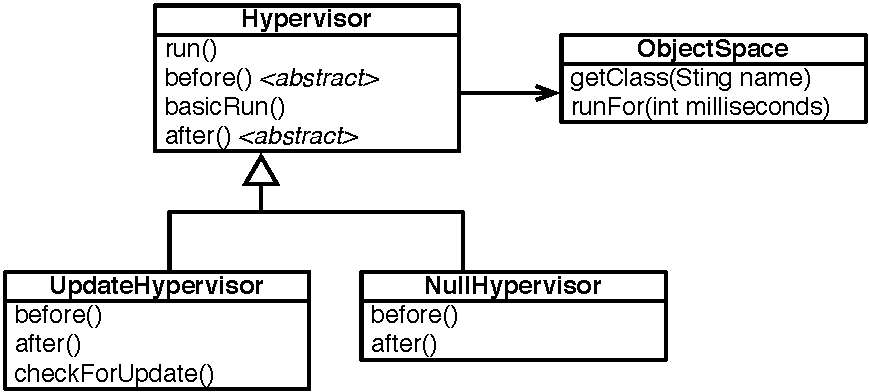
\includegraphics[width=.9\linewidth]{hypervisors}
\caption{\textbf{Example Hypervisors Class Hierarchy.} A \ct{NullHypervisor} does nothing while the \ct{UpdateHypervisor checks for updates before every cycle execution}.\label{fig:hypervisors}}
\end{figure}

\section{Cross-Runtime Communication} \label{sec:communication}\label{sec:isolation}

A hypervisor may require to apply some operation in a virtualized runtime that would be cumbersome through direct object manipulation with mirrors. Let's take as an example a virtualized application that uses a particular logging library where disabling logging means executing the following statement:

\begin{code}
Logger disable.
\end{code}

And the code invoked is:

\begin{code}
Logger class>>disable
	self uniqueInstance disable
	
Logger>>disable
	enabled := false
\end{code}

Doing the same through our abstract layer of mirrors presents the following drawbacks (a) to replicate the behavior of the \ct{disable} method inside the hypervisor and (b) to couple it to the internal representation of such a logging library. 

\begin{code}
OurHypervisor>>disableLogging
	logger := objectSpace getClass: #Logger.

	"the logger is a singleton"
	"in a class variable named uniqueInstance"
	loggerInstance := logger classVariableAt: #UniqueInstance.

	"The 'enabled' instance variable is the first"
	loggerInstange instanceVariableAt: 1 put: false.
\end{code}

A hypervisor may benefit from the execution of an arbitrary expression or statement within the scope of the virtualized runtime. It will reduce in this example the coupling to only the public API of the logging library. For example, enabling or disabling a logger from the virtualized application can be easily achieved through executing the following statement in the hypervisor instead of manually modifying the state of the logger objects:

\begin{code}
objectSpace execute: [ Logger disable ].
\end{code}

To achieve this kind of communication \Vtt provides two mechanisms: process injection and virtual interpretation.

\subsection{Process Injection}
The hypervisor and the virtualized runtime do not share core-libraries nor special objects, preventing us to easily perform a message-send between our co-existing application runtimes. Using the existing message-send mechanism provided by the \VM has the following challenges:

\begin{description}

\item[Cross-Runtime Method-Lookup.]A \emph{cross-runtime message-send}~(from the hypervisor to the virtualized runtime) cannot be simply achieved by a usual message-send mechanism. The usual message-send mechanism looks up in the receiver's class hierarchy a method with an \emph{object identical} method signature. However, our not-sharing strategy prevents the normal method-lookup work on a \emph{cross-runtime message-send} as symbols and classes are not shared between the different application runtimes. In such a case, the method-lookup mechanism fails because the elements of a message signature and the method signature we target are indeed \emph{equals but not identical}~(Figure \ref{fig:cross_runtime_lookup}).

\begin{figure}[ht]
\center
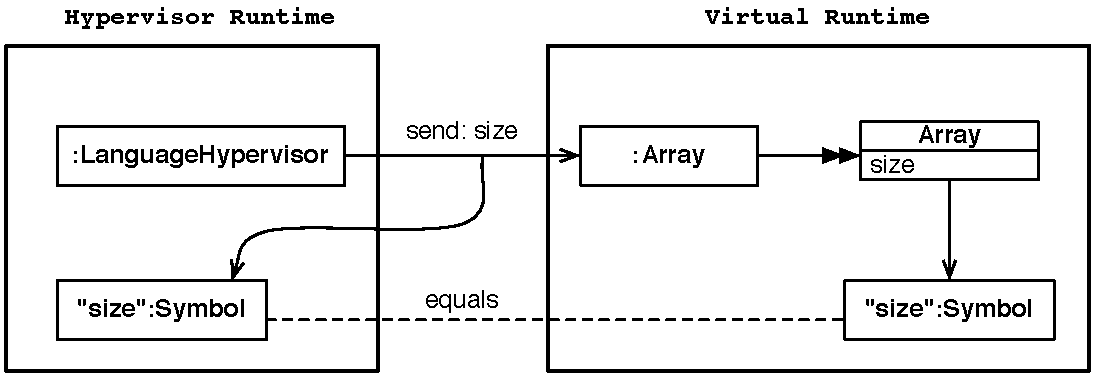
\includegraphics[width=.9\linewidth]{cross_runtime_lookup}
\caption{\textbf{Failing Cross-Runtime Method Lookup.} The hypervisor sends the \ct{size} message to an array in the virtualized runtime. This message-send signature is the hypervisor's \ct{size} symbol. The \ct{size} method exists but its signature has a different \ct{size} symbol. Both symbols are equals but not identical, and thus the lookup fails.\label{fig:cross_runtime_lookup}}
\end{figure}

\item[Exceptions and Stack.] A cross-runtime method-lookup succeeds if we modify the hypervisor message-send to contain the right symbol from the virtualized runtime. In such case, the execution stack contains a mixture of activations that belong to the hypervisor and the virtualized runtime. This poses a problem under the presence of techniques that traverse the execution stack indiscriminately, such as the exceptions or stack manipulation operations such as Smalltalk's \ct{thisContext} special variable. These operations may leak object references from an application runtime to another, leaving them in inconsistent state~(Figure \ref{fig:mixed_stack})~\cite{Mett10a}.

\begin{figure}[ht]
\center
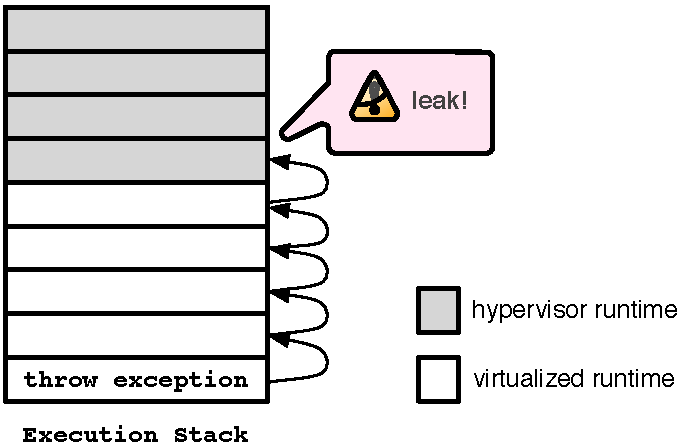
\includegraphics[width=.6\linewidth]{mixed_stack}
\caption{\textbf{Reference Leaks in a Mixed Stack on Exception.} When mixing the execution stack between the virtualized and hypervisor runtimes, an exception may traverse the stack and have access to a reference from a different application runtime.\label{fig:mixed_stack}}
\end{figure}

\end{description}

To overcome these problems we base the cross-runtime communication on \emph{process injection} \ie we create a new thread inside the virtualized runtime containing the expression to execute. This new thread executes in cycles until it is finished. Once finished, from the hypervisor we can access the result of the execution through a mirror on the process~(cf. Figure \ref{fig:process_injection}).

\begin{figure}[ht]
\center
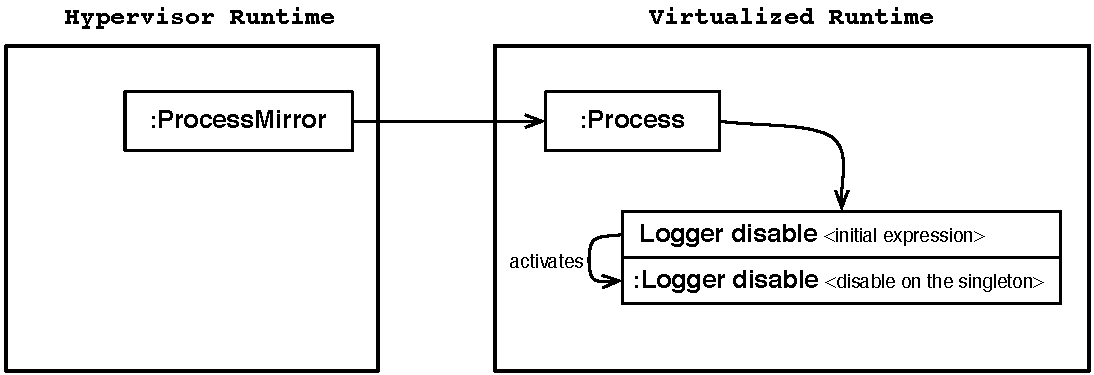
\includegraphics[width=.9\linewidth]{process_injection}
\caption{\textbf{Process injection.} The hypervisor can install and manipulate a process through a mirror. The result can accessed from the mirror.\label{fig:process_injection}}
\end{figure}

To perform process injection, we need to marshall the arguments, literals and the returned object between their representation in the hypervisor from/to their equivalent representation in the virtualized runtime. For example, marshaling a \ct{String} object means to create a new \ct{String} object in the other application runtime with its corresponding class and copying all its bytes. Global object references such as classes are mapped to their corresponding mirrors in the virtualized runtime. Non-global non-literal objects can be specified explicitly as an argument with their corresponding mirrors.

\begin{code}
objectSpace
	execute: [ :aLogger | aLogger disable ]
	with: aLoggerInstanceMirror.
\end{code}

This solution for cross-runtime communication solves both problems observed before. In a first place, it prevents the method-lookup failure by translating the objects part of the method signature. Second, the new process executes in its own stack ensuring none of the objects from the hypervisor are leaked to the virtualized runtime.

\subsection{Virtual Interpretation} \label{sec:interpretation}

It may happen that a virtualized runtime is in an state where it cannot execute code by itself. An virtualized runtime may be in a buggy state due to a change, or it may be under construction (as in the subject of this thesis). In those cases, we cannot delegate the execution to the virtualized runtime itself and thus, we cannot use the process injection mechanism. Let's for example consider that we accidentally break or remove the \ct{at:put:} method from the \ct{MethodDictionary} class. Since that method is the one used to install new methods, from that moment on we cannot install methods in classes using process injection any more. Moreover, solving this problem would require to install a method, preventing us to do it through process injection.

\begin{code}
methodDictionaryClass := objectSpace classNamed: #MethodDictionary.
methodDictionaryClass remoteMethod: #at:put:.

"now we cannot install methods using process injection any more"
\end{code}

For such cases \Vtt allows us to execute an expression inside a virtualized runtime within the context of the hypervisor through the \emph{virtual interpretation} of \eg abstract syntax trees~(ASTs) or bytecodes. A virtual interpreter is a first-class entity that resides inside the hypervisor and interprets code inside a virtualized runtime. As it is a first-class entity, we can easily modify its implementation details such as the method lookup or the execution of primitives. These kinds of modifications allow us to handle the special cases that cannot be handled by process injection. Then, we can use a virtual interpreter to execute an AST equivalent to the \ct{at:put:} method to install back our corresponding method. This puts the virtualized runtime in our example back into a stable state before it can continue its own execution.

\begin{code}
"newMethod is a method that fixes the bug"
newMethod := objectSpace compileMethod: 'at: aKey put: aMethod ....'.

interpreter := VirtualInterpreter newOn: anObjectSpace.
interpreter
	execute: [ Object methodDictionary at: #brokenSelector put: newMethod ]
	with: newMethod.
	
"now we can continue working with process injection"
\end{code}

% =============================================================================
\section{Conclusion and Summary}

\Vtt presents an architecture where several application runtimes can share the same process. A virtualized application runtime is subject to monitoring and manipulation from another application runtime, namely the hypervisor runtime. The hypervisor runtime contains a first class representation of the virtualized runtime, namely an object space. The object space exposes a clear interface to safely access and modify an application runtime. This interface includes operations to configure the virtualized application runtime and operations to modify particular objects from it. The latter is encapsulated in mirror objects.

The execution of a virtualized runtime is organized in cycles. In between cycles, the hypervisor can perform an operation and then resume the virtualized runtime execution. We ensure that the state of the virtualized runtime keeps its coherence by only suspending it in safe suspension points.

Besides the direct manipulation through mirrors, a hypervisor can perform cross-runtime message-sends for a richer communication using process injection. Process injection prevents failures in the method lookup and avoids stack traversing techniques such as exception to leak cross-runtime references. Additionally, a virtual interpreter allows us to execute code in the virtualized runtime with full intercession. A virtual interpreter is a first class entity, allowing us to easily specialize and change it.

In following chapters we will show our prototype implementation of this infrastructure and how this infrastructure supports the evolution of a programming application runtime in two different scenarios. First, the recreation of a application runtime using an explicit bootstrap process. Second, an application tailoring technique that specializes an application runtime to contain only elements that are used during runtime.

\input{chapter-footer.tex}